\documentclass[12pt]{report}
\usepackage[margin=1in]{geometry}
\usepackage{setspace} % for single/doublespacing commands
\usepackage{graphicx} % including graphics
\usepackage{sectsty} % sexy section headings
\usepackage{pdfpages} % including multipage pdfs
\usepackage[export]{adjustbox} % for graphic frames and center
\usepackage{siunitx}
\usepackage[numbered]{matlab-prettifier} % including matlab w/ syntax highlighting
\usepackage[T1]{fontenc} % prettier matlab font
\usepackage{xfrac} % more legible inline fractions (\sfrac)
\usepackage{lmodern} % font package for above
\usepackage{multicol} % multiple columns
\usepackage[justification=centering]{caption} % figure captions (force centering)
\usepackage{amsmath} % more math symbols and shit
\usepackage{enumitem} % add arguments for enumerate to change style
\usepackage[list=true]{subcaption} % subfigures with list of figure support
\usepackage{multirow}
\usepackage{mathtools}
\usepackage{booktabs}
\usepackage{color}
\usepackage{ulem}
\usepackage{blindtext}
\usepackage[numbers]{natbib}
\usepackage{contour}
\usepackage{tabularx}
\usepackage{circuitikz} % drawing fancy shit
\usepackage{cancel} % arrow and cross math cancel symbol
\usepackage{lineno}
\usepackage{framed}
\usepackage{amssymb} % special math symbols
\usepackage{listings}
\usepackage{array}
\usepackage{BOONDOX-cal} % fancy mathtype script
\usepackage{fancyhdr}
\usepackage{flowchart}
\usepackage{color, colortbl}
\usepackage{tocloft}
\usepackage{url}
\usepackage{etoolbox}

\setlength{\parskip}{\baselineskip}%
\setlength{\parindent}{0pt}%
\setcounter{secnumdepth}{5}
\renewcommand{\bibname}{References}
\sisetup{output-exponent-marker=\ensuremath{\mathrm{e}}}
\newcommand{\PreserveBackslash}[1]{\let\temp=\\#1\let\\=\temp}
\newcolumntype{C}[1]{>{\PreserveBackslash\centering}p{#1}}
\newcolumntype{R}[1]{>{\PreserveBackslash\raggedleft}p{#1}}
\newcolumntype{L}[1]{>{\PreserveBackslash\raggedright}p{#1}}
\lstMakeShortInline[style=Matlab-editor]| % matlab inline escape character
\graphicspath{{images/}}
\renewcommand\thesection{\arabic{section}}
\renewcommand\labelitemi{---}
\lstset{numberstyle=\ttfamily\small\color{gray}}
\renewcommand\linenumberfont{\ttfamily\small\color{gray}}
\setlength\linenumbersep{6mm}
% \hbadness=99999  % or any number >=10000
\apptocmd{\sloppy}{\hbadness 10000\relax}{}{}
% \usetikzlibrary{arrows,calc,patterns,angles,quotes}
% \usetikzlibrary{shapes.geometric}
% \usetikzlibrary{decorations.pathmorphing,decorations.pathreplacing} % for snakes!
% \usetikzlibrary{positioning, circuits.logic.US}

\setlength{\cftbeforetoctitleskip}{-2em}
\newcommand{\Lag}{\mathcal{L}} % lagrangian L
\begin{document}
\normalem
\begin{titlepage}
\flushleft
\doublespacing
\Large
\textsc{Test Document} \\
\normalsize
Trey Dufrene, Zack Johnson, David Orcutt, Alan Wallingford, Ryan Warner
\vfill
\center
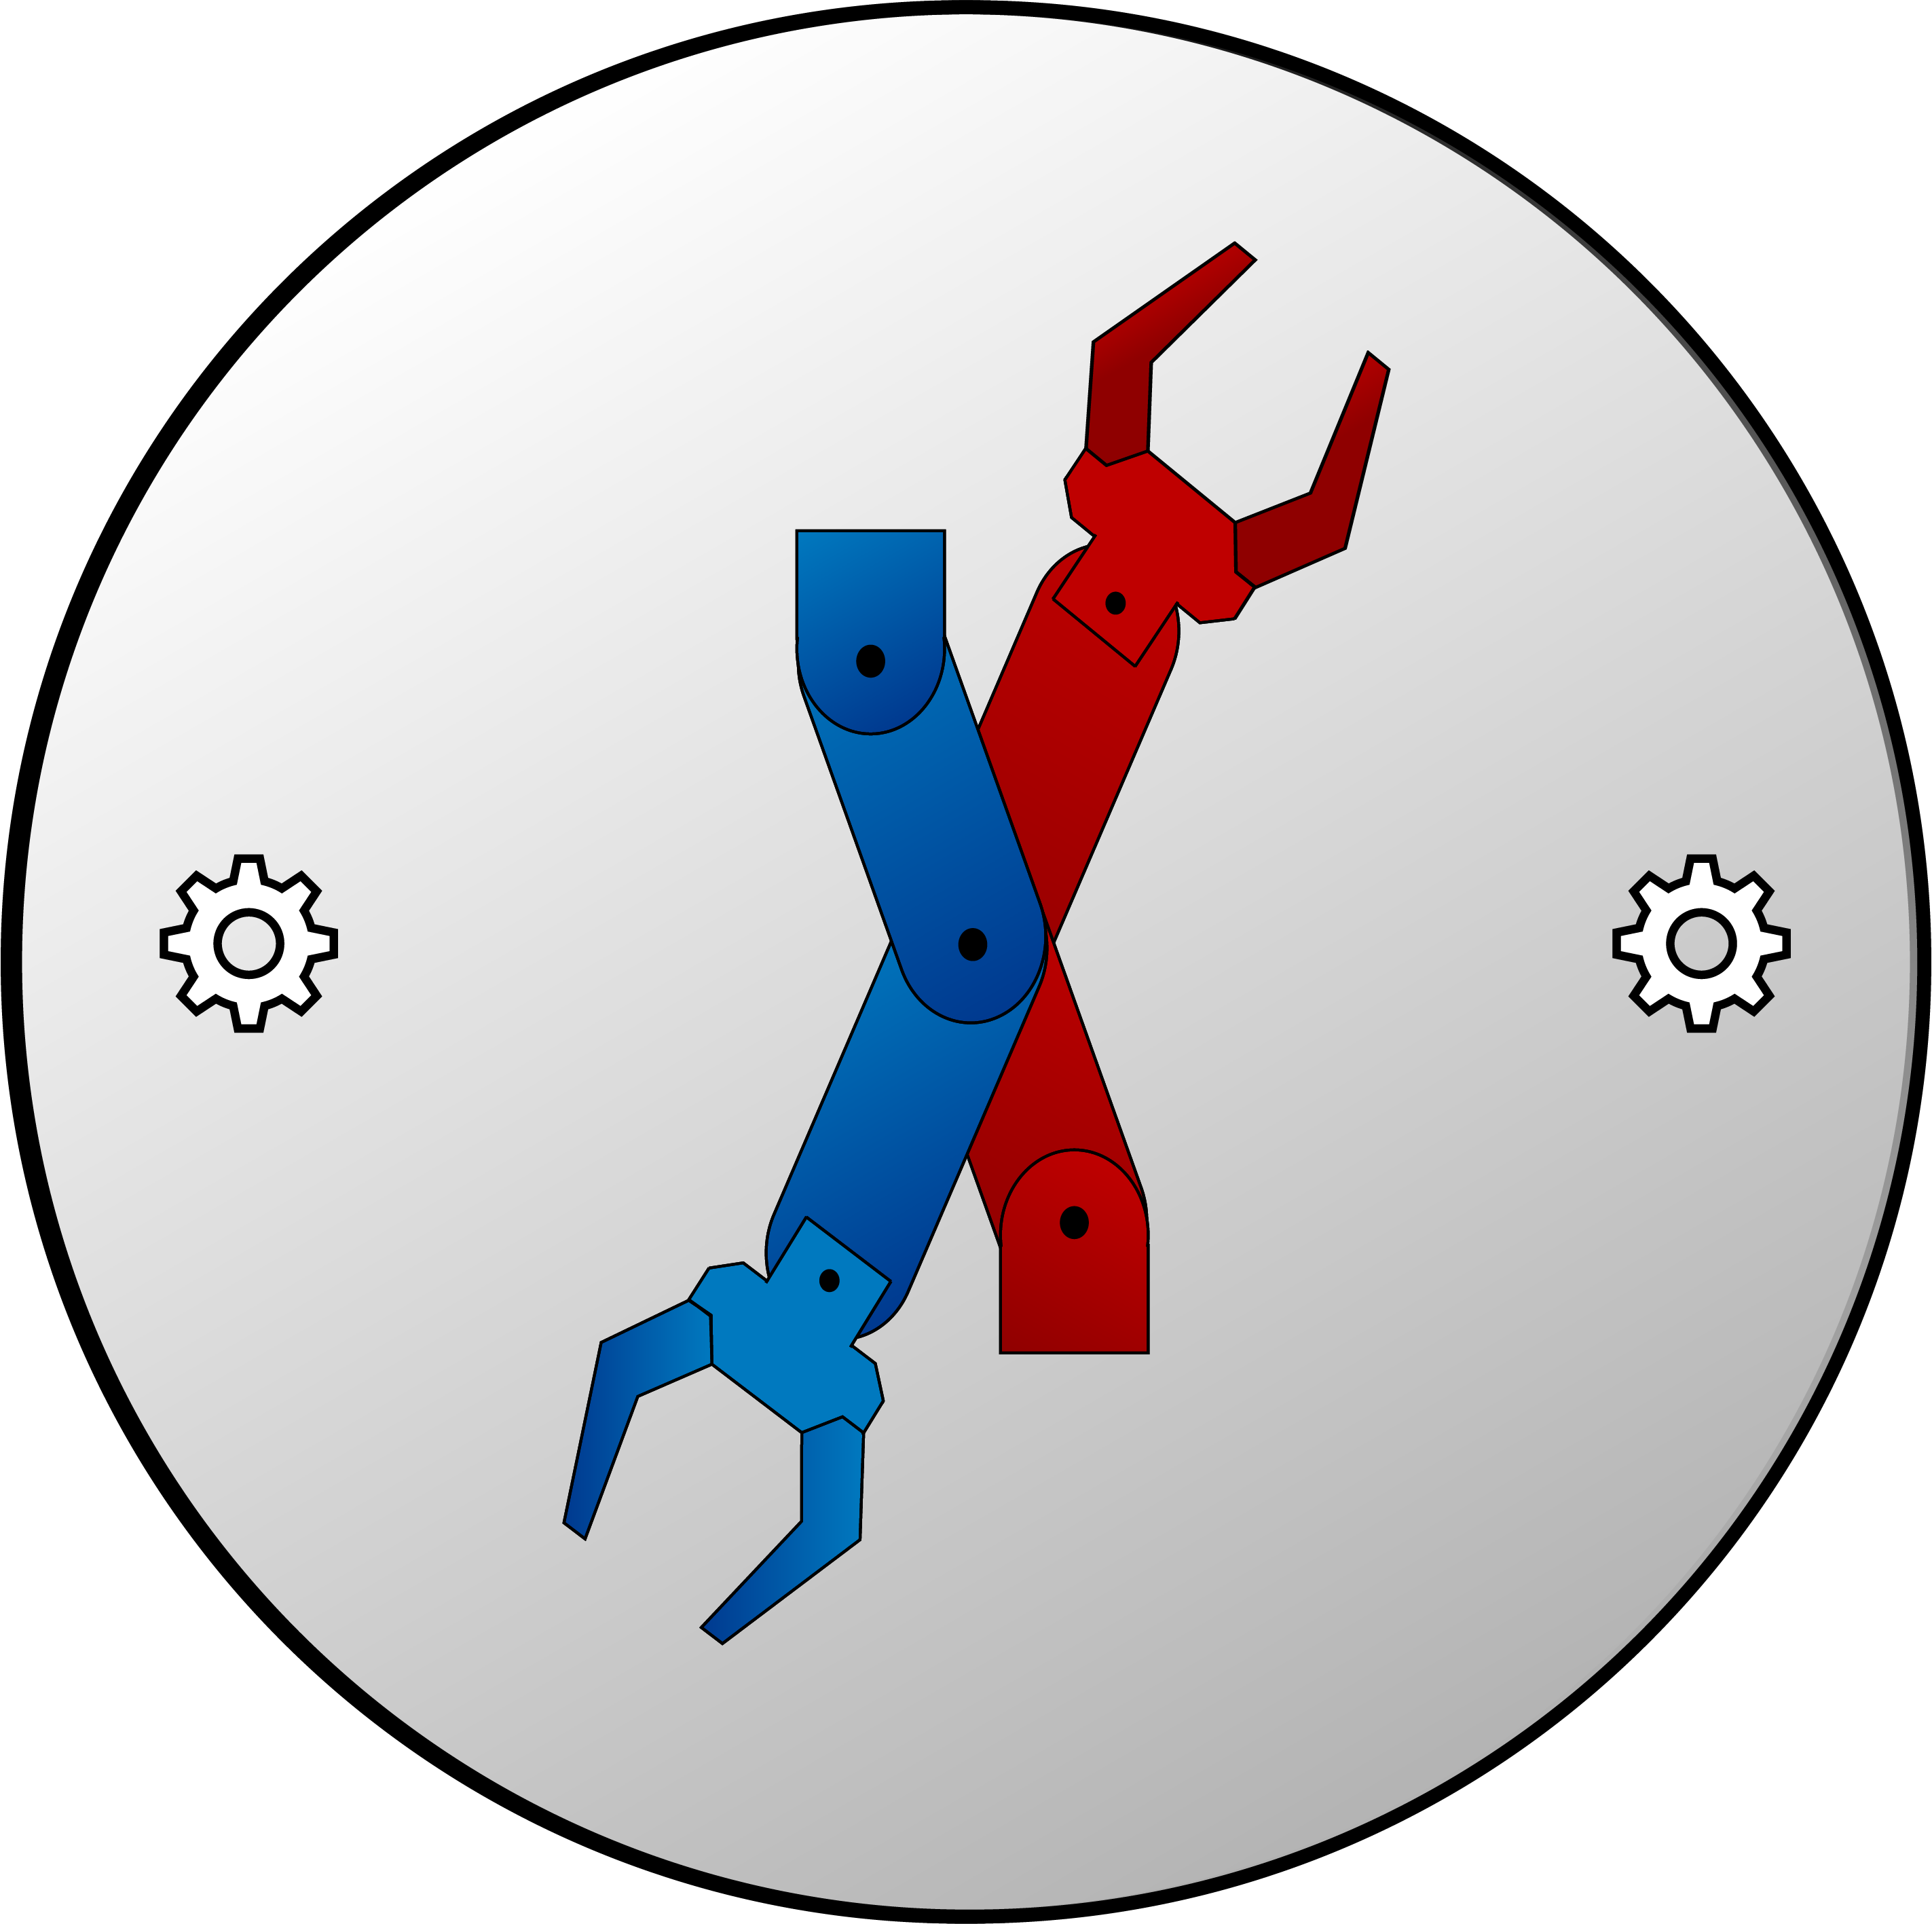
\includegraphics[width=.45\textwidth]{logo}
\vfill
\flushleft
ME 407 \\
Preliminary Design of Robotic Systems \\
Embry-Riddle Aeronautical University \\
\vspace{2ex}
\begin{minipage}[c]{.5\textwidth}
\flushleft

\includegraphics[width=.95\textwidth]{erau}
\end{minipage}%
\begin{minipage}[c]{.5\textwidth}
\flushright

\includegraphics[width=.8\textwidth]{text}
\end{minipage}
\end{titlepage}

\pagenumbering{roman}
% \begin{abstract}
  % Wordy words
% \end{abstract}
{\tableofcontents\let\clearpage\relax\listoffigures\let\clearpage\relax\listoftables}
\clearpage
\newpage

% \section*{List Of Acronyms and Abbreviations}

% \begin{tabular}{rl}
%   $G$~:&Center of gravity of the bar \\
%   $\ell_0$~:& Spring unstretched length  \\
%   $\delta$~:& Spring deflection \\
%   $k$~:& Spring constant \\
%   $h_{b}$~:& Distance to bar ($G$) from datum \\
%   $F_s$~:& Force onto bar due to spring\\
%   $A_{n}$~:& Pin reaction in $\theta$ direction\\
%   $A_{t}$~:& Pin reaction in tangential direction \\
%   $\vec{v}_G$~:& Velocity of bar center of gravity\\
%   $\ddot{\theta}$~:& Angular velocity of spring \\
%   $\ddot{\phi}$~:& Angular velocity of bar\\
%   $\ddot{\ell}_s$~:& Radial acceleration of spring \\
% \end{tabular}
% \normalsize
% \flushleft
% \singlespacing
% \newpage

\pagenumbering{arabic}
\onehalfspacing
\section{Introduction}
\vspace{-.75\baselineskip}
The terminator T-2000 is a science-fiction spectacle of a robot -- until you see the price. Channeling the inspiration many high school students may have for robotics, MEIOSIS robotics aims to provide an affordable manipulator to educators and enthusiasts. MEIOSIS uses primarily 3-D printed components and easily accessible materials. Among these materials are a Raspberry PI, smart servos and metal tubing. These features create an open-source manipulator accessible to the public to further robotics education.

\section{Physical System Overview}
\vspace{-.75\baselineskip}
The physical design of the robotic manipulator will be shown through Figures \emph{\ref{fig:overall}, \ref{fig:base}, \ref{fig:link1},} and \emph{\ref{fig:link2}}.

\begin{figure}[htp]
  \centering
  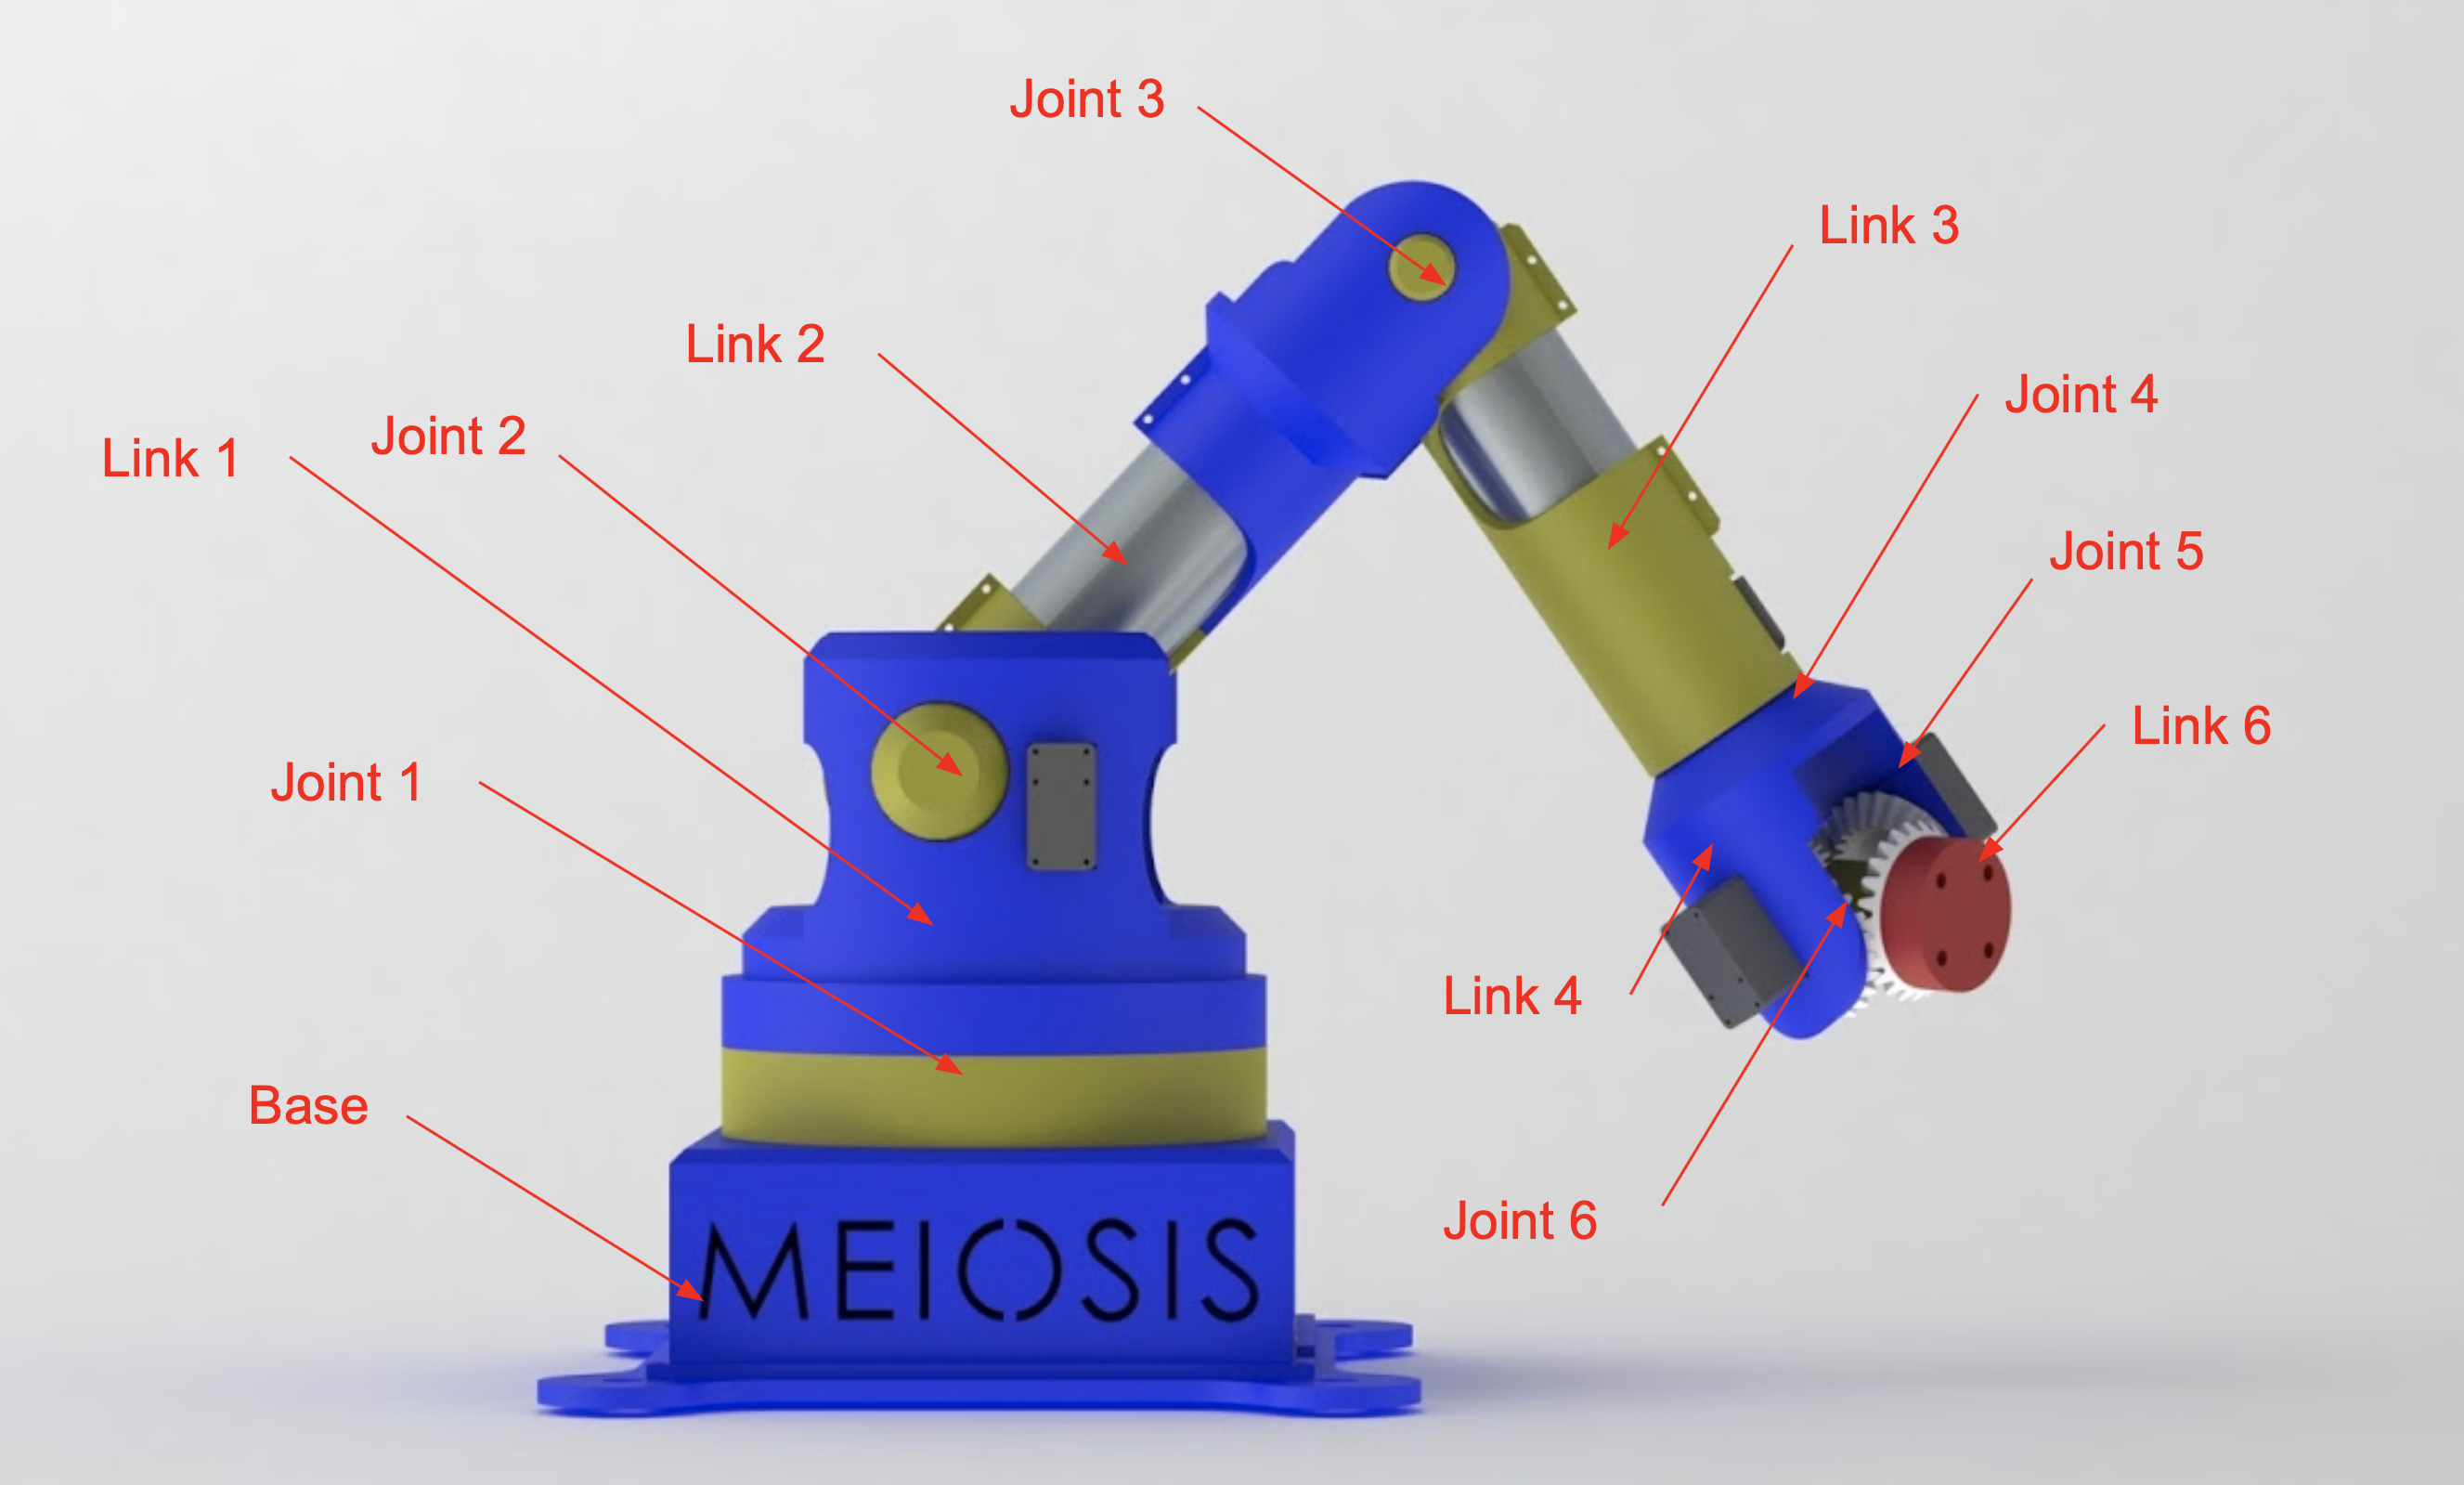
\includegraphics[frame, width=.75\textwidth]{overall_render}
  \caption{Overall System Conceptual Design }
  \label{fig:overall}
\end{figure}

The colored links in \emph{Figure \ref{fig:overall}} distinguish the different joints and links of the manipulator. The overall reach of the robot will be 582.5 mm. This length was chosen to decrease material cost and weight while still satisfying requirement 2.1.2 and 2.1.5, allowing the manipulating to pick and place objects to perform basic tasks. The base of the robot will be made to contain the Raspberry Pi and other electrical components.
\newpage
\subsection{Base}
The base of the manipulator will house several of the electronic components, such as the computational system, power supply, and motor controller. A cross section of the base can be seen in \emph{Figure \ref{fig:base}}.
\begin{figure}[htp]
  \centering
  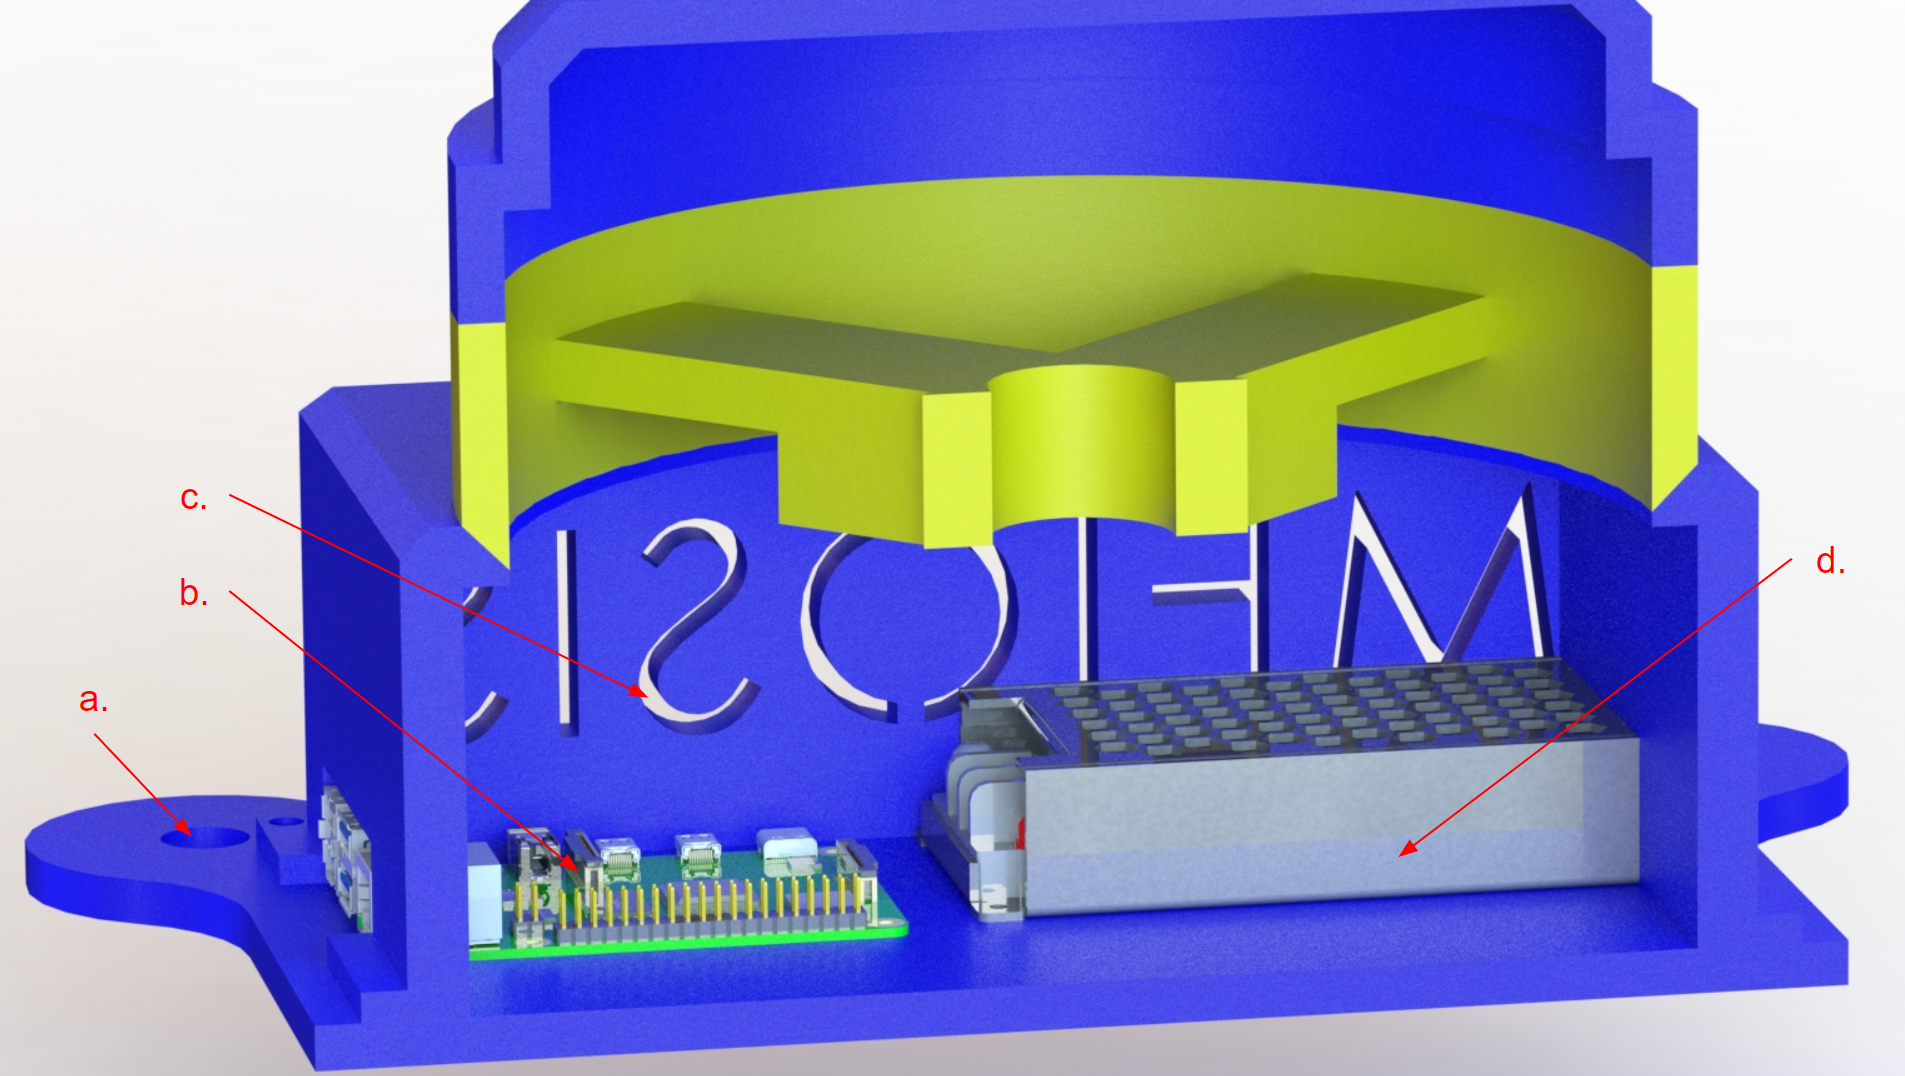
\includegraphics[frame, width=.75\textwidth]{base_callouts}
  \caption{Manipulator Base with Call-outs}
  \label{fig:base}
\end{figure}

From \emph{Figure \ref{fig:base}},
\vspace{-\baselineskip}
\begin{enumerate}[label=\alph*.]
  \item \emph{Base Supports:}
  The base supports are located at each corner of the base and will allow the base of the manipulator to be securely attached to a variety of surfaces with either standard bolt/fastener hardware or suction cups.
  \item \emph{Computational System:}
  The computational system will be a Raspberry Pi; it will be housed in the base, which allows the Raspberry Pi to be more easily accessible. The primary reason for this system being chosen is to fulfill the budget requirement, 2.1.1. The Raspberry Pi will compute the manipulator's kinematics and command the motors accordingly.
  \item \emph{Airflow Cutouts:}
  The side of the base will have cutouts to allow for airflow through the base; since the power supply is housed inside of the base as well as the computational system, the temperature must be regulated to prevent overheating.
  \item \emph{Power Supply:}
  The power supply will be housed in the base as well; this allows the power supply to be more accessible and therefore more modifiable, so the end-user can easily expand the system to fulfill their needs.
\end{enumerate}
\subsection{Links}
\emph{Figure \ref{fig:link1}} is an image of the robot that shows the links and their key features.\\
\begin{figure}[htp]
  \centering
  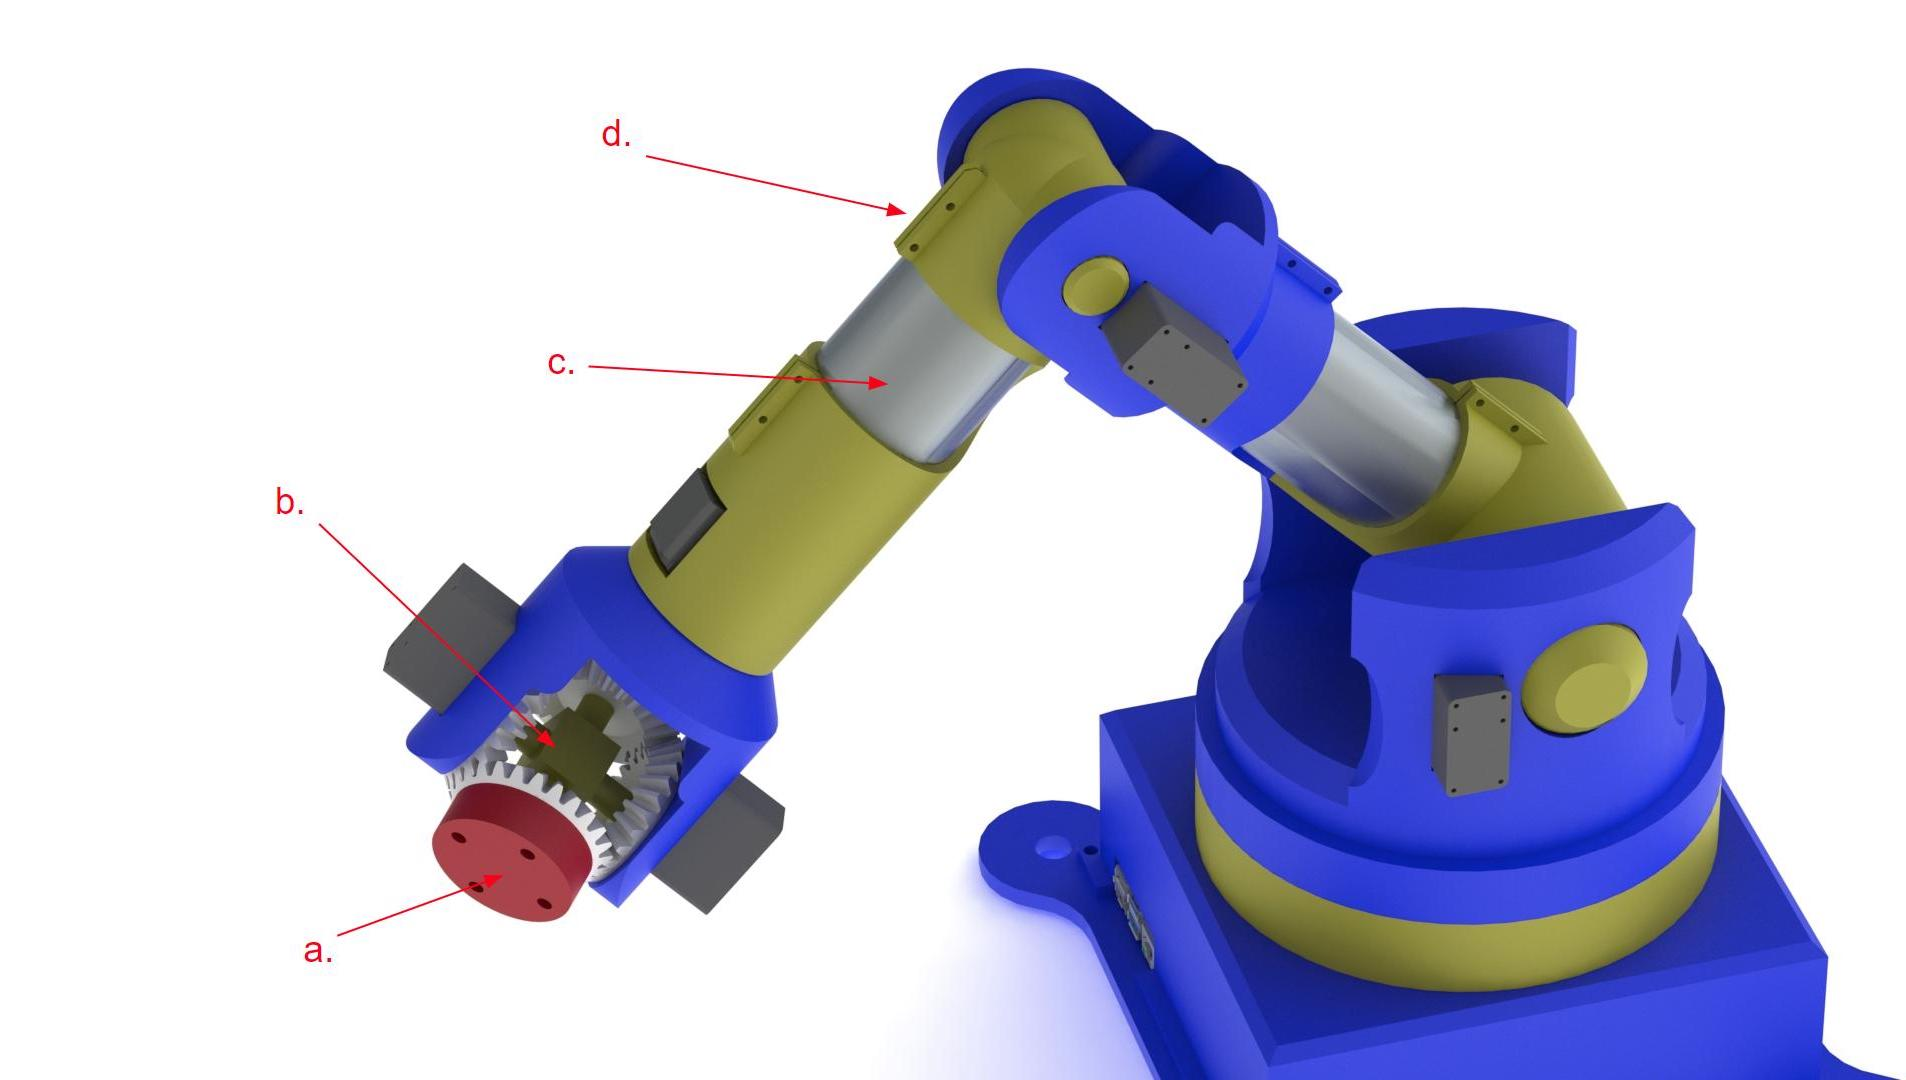
\includegraphics[frame,width=.63\textwidth]{link_callouts}
  \caption{Drawing Showing Key Features of Design}
  \label{fig:link1}
\end{figure} \\
\emph{Figure \ref{fig:link1}} highlights a few of the key features of our design. Call-out a shows the connection point for the end effector. The mountings are the standard used by the Sawyer manipulator. This may be adjusted to accommodate lower cost, more accessible end effectors. Call-out (b) shows the differential gearbox that will be used in the manipulator’s wrist, saving space and weight. The manipulator will have aluminum tubing as support in the links (c) and will be attached to the 3D printed portion of the robot using clamp joints (d) tightened by screws.

\emph{Figure \ref{fig:link2}} is an image of the cross section of link 2 for the manipulator.
\begin{figure}[htp]
  \centering
  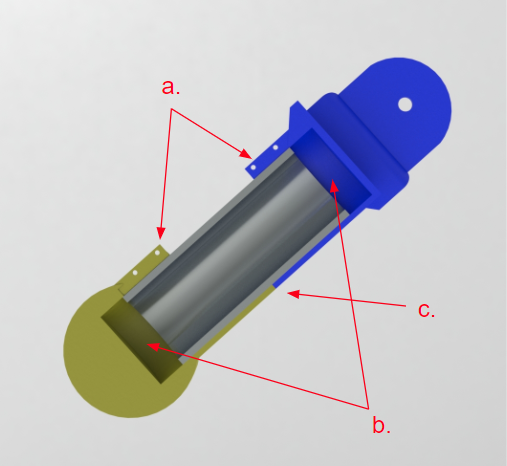
\includegraphics[frame,width=.35\textwidth]{link_cross_section}
  \caption{Drawing Showing Link Cross Section}
  \label{fig:link2}
\end{figure}
\newpage
The cross section seen in \emph{Figure \ref{fig:link2}} shows the internal design for links two and three. It features two clamps that hold a hollow aluminum bar in place (a) and allows for gaps between the aluminum tube and the 3D printed call-out (b). The proper length will be dictated by the 3D printed guides lining up at call-out (c). This allows for imprecision in the manufacturing of the aluminum tube.

\section{System Functions}
The system can be divided into two subsystems: the electrical and software systems. The electrical subsystem includes the wiring and hardware computational components, power system, actuators with drivers, and sensors. The software subsystem includes the algorithm for the computational system.
\subsection{Electrical}
\emph{Figure \ref{fig:eblock}} is the block diagram for the electrical system of the manipulator.

\begin{figure}[htp]
  \centering
  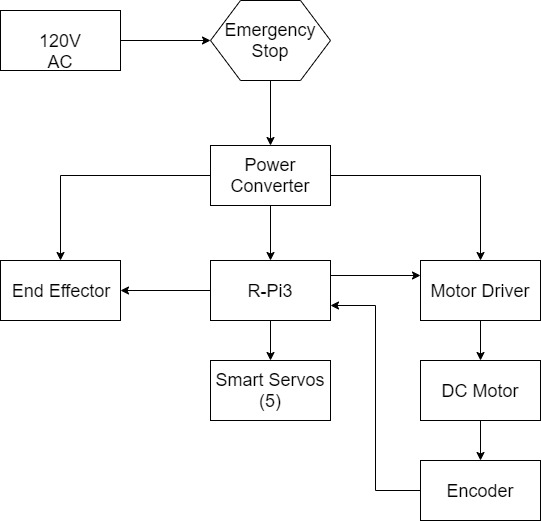
\includegraphics[width=.55\textwidth]{eblock}
  \caption{Electrical System Block Diagram}
  \label{fig:eblock}
\end{figure}

\emph{Figure \ref{fig:eblock}} shows that the electrical systems of the manipulator will be relatively simple. Power is supplied by the 120V AC from standard wall outlets. A power supply will adapt the AC voltage to the required voltages for each component. One component is the Raspberry Pi, which will perform calculations for motor control (described below in software). It will send signals to the DC motor driver and the five smart servos. The smart servos have an on-board controller, so no feedback will be necessary. However, the first joint, between the base and the first link, will be actuated by a DC motor with an encoder to minimize cost.

\subsection{Software}
\emph{Figure \ref{fig:sblock}} shows the software flowchart for the system.
\begin{figure}[ht]
  \centering
  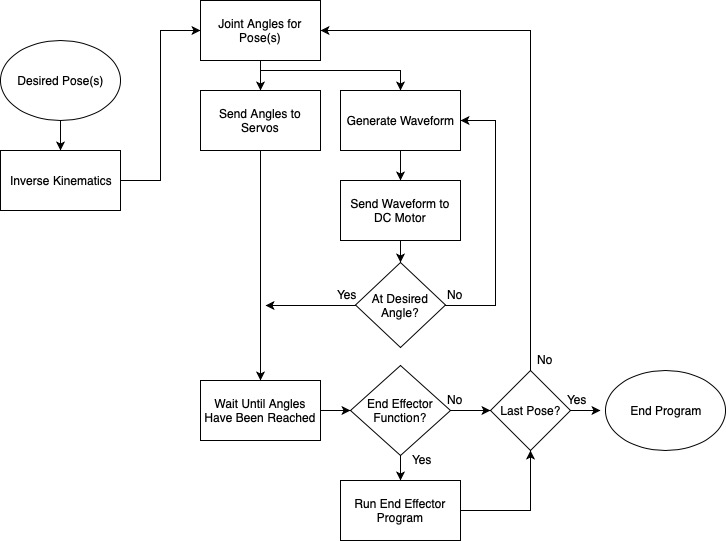
\includegraphics[width=.85\textwidth]{sblock}
  \caption{Software Flowchart}
  \label{fig:sblock}
\end{figure}

Similar to the electrical system, the software is also simple. \emph{Figure \ref{fig:sblock}} shows that the software will receive the desired pose or poses the user would like the manipulator to reach. Then the Raspberry Pi will use inverse kinematics to calculate the necessary joint angles. The wave-forms/desired angles will be sent to the respective drivers/motors, and positional information will be sent back to the Raspberry Pi to adjust the DC motor angle. When the motors have reached their desired pose, the Raspberry Pi will actuate the end effector if it is specified by the user. The system will then check to see if there are any more poses to reach and either repeat the motor control section given the desired angles of the new pose or end program if the last pose has been reached.

\section{Parts List and Manufacturing}
Our costs are estimated from all specific components we envision requiring with a factor of safety. The 20\% factor of safety is the sum of 20\% of the cost for each item listed in Table 4.1 and is intended to account for shipping, taxes, and replacement/additional parts. Including this factor of safety, we satisfy requirement 2.1.1 with a predicted budget of \$798.80.

\begin{table}[htp]
  \center
  \caption{Predicted List of Parts}
  \label{table:costs}
  \begin{tabular}{C{3.5cm}C{3cm}C{1.5cm}|C{1.5cm}c}
  \multirow{2}{*}{\textbf{Part}} & \textbf{Unit Cost (USD)} & \multirow{2}{*}{\textbf{Qty}} & \textbf{Cost (USD)} & \multirow{2}{*}{\textbf{Source}} \\ \hline
  2kg PLA & 32 & 1 & 32 & Amazon \\
  Smart Servo & 140 & 2 & 280 & Trossen Robotics \\
  Lower Torque Smart Servo (6 pack) & \multirow{3}{*}{225} & \multirow{3}{*}{1} & \multirow{3}{*}{225} & \multirow{3}{*}{Trossen Robotics} \\
  DC Motor w/ Encoder & \multirow{2}{*}{30} & \multirow{2}{*}{1} & \multirow{2}{*}{30} & \multirow{2}{*}{Robot Shop} \\
  Power Supply & 16 & 1 & 16 & Compt. Dist. Inc. \\
  Raspberry Pi 3 & 35 & 1 & 35 & Adafruit \\
  3 Pin Cables & 9 & 1 & 9 & Amazon \\
  4 Pin Cables & 13 & 1 & 13 & Amazon \\
  Gripper & 25 & 1 & 25 & Trossen Robotics \\
  &&&\\
  Factor of Safety (20\%) & & & \multirow{2}{*}{133} & \\
  & & \textbf{Total} & \$798 & \\
  \end{tabular}
\end{table}

Our motor costs are approximated from three motor types. For use in joint one is one stepper motor \cite{robotis}. It should experience minimal torque from gravity acting on the other links and does not require a continuous voltage to maintain position. The built-in encoder provides feedback for accurate motion and limiting the rotation to 2$\pi$ radians. For use in joints 2 and 3 are two smart servos with holding torque of 1.6N$\cdot$m. These feature a built in PD control, which means no overshooting, that can be precise to 0.29\(^{\circ}\) with tuning \cite{matterhackers}. So long as the links, servos, and payload after the base do not exceed 0.65kg acting through the horizontally outstretched arm’s centroid, 250mm from the base, the torque is sufficient. Although the servos are continuous rotation, joints 2 and 3 are not free to rotate \(360^{\circ}\) and will be limited by software. Finally, for the spherical wrist are three lower cost, lower torque, smart servos which also have PD control and a \(0.29^{\circ}\) resolution \cite{rev}. The gripper will also be actuated with one of these servos.

Since each motor has the same voltage requirement of 12V and our manipulator is powered by 120V AC, we also account for the cost of a power supply. The power and communication buses are handled by four pin wires for the smart servos and three pin wires for the lower-cost smart servos. 2kg of PLA filament allows all components of the manipulator to be 3D printed with 100\% infill, making it an overestimate. With a 20\% factor of safety to account for shipping, taxes, and unexpected part purchases, we are under our team budget of \$800 and design budget of \$1000.

\emph{Table \ref{table:gantt}} shows the Gantt chart for the remainder of the fall semester.
\definecolor{Gray}{gray}{0.5}
\definecolor{DGray}{gray}{0.4}

\begin{table}[htp]
  \center
  \caption{Gantt Chart}
  \label{table:gantt}
\begin{tabular}{C{2.9cm}|cccccccccccccccccc}
& \multicolumn{18}{c}{ Class Work Session } \\ 
\textbf{Software} \small & 1 & 2 & 3 & 4 & 5 & 6 & 7 & 8 & 9 & 10 & 11 & 12 & 13 & 14 & 15 & 16 & 17 & 18 \\\hline\normalsize
Kinematics & \cellcolor{DGray} & \cellcolor{DGray} & \cellcolor{DGray} & \cellcolor{DGray} & \cellcolor{DGray} & & & & & & & & & & & & & \\
Microcontroller Compatability & \cellcolor{Gray} & \cellcolor{Gray} & & & & & \cellcolor{Gray} & \cellcolor{Gray} & & & & & & & & & & \\
Motor Actuation & & \cellcolor{DGray} & \cellcolor{DGray} & \cellcolor{DGray} & \cellcolor{DGray} & \cellcolor{DGray} & \cellcolor{DGray} & \cellcolor{DGray} & & & & & & & & \cellcolor{DGray} & \cellcolor{DGray} & \cellcolor{DGray} \\
\textbf{Motors} & & & & & & & & & & & & & & & & & & \\\hline
Model & & & & & & & & & \cellcolor{Gray} & \cellcolor{Gray} & \cellcolor{Gray} & \cellcolor{Gray} & \cellcolor{Gray} & \cellcolor{Gray} & & & & \\
Calibration & & & & & & & & & & & & & & & & \cellcolor{DGray} & \cellcolor{DGray} & \cellcolor{DGray} \\
Interfacing & & & & & & & & & & & & & \cellcolor{Gray} & \cellcolor{Gray} & \cellcolor{Gray} & \cellcolor{Gray} & & \\
\textbf{Links} & & & & & & & & & & & & & & & & & & \\\hline
Model & & & & \cellcolor{DGray} & \cellcolor{DGray} & \cellcolor{DGray} & \cellcolor{DGray} & \cellcolor{DGray} & \cellcolor{DGray} & & & & & & & & & \\
Print & & & & & & & & \cellcolor{Gray} & \cellcolor{Gray} & \cellcolor{Gray} & \cellcolor{Gray} & \cellcolor{Gray} & & & & & & \\
\textbf{Wiring} & & & & & & & & & & & & & & & & & & \\\hline
Bus Testing & & \cellcolor{DGray} & \cellcolor{DGray} & \cellcolor{DGray} & & & & & & & & & & & & & & \\
Mapping & & & & & & & & & \cellcolor{Gray} & \cellcolor{Gray} & \cellcolor{Gray} & \cellcolor{Gray} & \cellcolor{Gray} & & & & & \\
Implementation & & & & & & & & & & & & & & \cellcolor{DGray} & \cellcolor{DGray} & \cellcolor{DGray} & \cellcolor{DGray} & \cellcolor{DGray} \\
\textbf{Manipulator} & & & & & & & & & & & & & & & & & & \\\hline
Link Fitting & & & & & & & & & & & & \cellcolor{Gray} & \cellcolor{Gray} & \cellcolor{Gray} & \cellcolor{Gray} & & & \\
Calibration & & & & & & & & & & & & & & & & \cellcolor{DGray} & \cellcolor{DGray} & \cellcolor{DGray} \\
Gripper Interchangability & & & & & & & & & & & & & & \cellcolor{Gray} & \cellcolor{Gray} & & & \\
\end{tabular}
\end{table}


\emph{Table \ref{table:gantt}} shows approximately half our time for Fall semester will be used modeling the manipulator’s kinematics, motor dynamics, and physical links with the second half dedicated to interfacing parts, wiring, and testing components. Nonetheless, the manipulator should have a functional guise by the semester’s end, however, we anticipate our design will require further iterations before it satisfies all our requirements. For example, a refined control interface usable by novice robotics students is not accounted for.

\section{Decision Matrices}
The design for the end effector attachment varied across each of the team member’s original conceptual designs, therefore a decision matrix was constructed to objectively decide on the best design for the manipulator.

\begin{table}[htp]
  \center
  \caption{End Effector Attachment Design Decision Matrix}
  \label{table:ee}
\begin{tabular}{C{3.5cm}|cccc}
\textbf{EE Attachment} & \textbf{Ease of Use} & \textbf{Manufacturability} & \textbf{Durability} & Total \\
Weighting & 3.6 & 5 & 7 & \\\hline
Screw Connections & 6.8 & 8.8 & 9.8 & \textbf{137.08} \\
Snap Fit Joint & 8.6 & 5 & 2.2 & 71.36 \\
Threaded End Effector & 6.3 & 5.4 & 7.3 & 100.78 \\
\end{tabular}
\end{table}

As shown in \emph{Table \ref{table:ee}}, the optimal design must be somewhat easy to use, easily manufacturable, and the most durable. This is the best represented by the screw connections design.

\begin{table}[htp]
  \center
  \caption{Material Choice Decision Matrix}
  \label{table:mat}
\small\begin{tabular}{c|cccccc}
\textbf{Material} & \textbf{Cost} & \textbf{Weight} & \textbf{Accessibility} & \textbf{Manufacturability} & \textbf{Durability} & Total \\\normalsize
Weighting & 9.2 & 6.6 & 8 & 6.4 & 5.4 & \\\hline
3D Printed & 8 & 9 & 8 & 9.4 & 5 & 284.16 \\
Aluminum & 4 & 5.8 & 5.8 & 6.6 & 9.2 & 213.4 \\
Combination & 8 & 7.8 & 7 & 9 & 9.2 & \textbf{288.36} \\
\end{tabular}
\end{table}
As seen in \emph{Table \ref{table:mat}}, the primary material chosen to create the manipulator is PLA / 3D printed material, this is due to its low cost and accessibility; additionally, it is lightweight, manufacturable, and durable. Further, by using primarily 3D printed parts, the end-user’s cost is potentially lower and their ability to modify parts is enhanced.
\newpage
\begin{table}[htp]
  \center
  \caption{Computing Choice Decision Matrix}
  \label{table:comp}
\begin{tabular}{c|ccccc}
\textbf{Computing System} & \textbf{Cost} & \textbf{Capabilities} & \textbf{Ease of Use} & \textbf{Independance} & Total \\
Weights & 10 & 4.2 & 7.6 & 4.2 & \\ \hline
RPi & 7.9 & 6 & 9 & 10 & \textbf{214.6} \\
Jetson & 1 & 7 & 7 & 9 & 130.4 \\
RPi + Arduino & 4.8 & 7 & 8 & 10 & 180.2 \\
Arduino & 9 & 4 & 9 & 3 & 187.8 \\
B Black & 1.2 & 7 & 7 & 10 & 136.6 \\
B Green & 5 & 7 & 6 & 9 & 162.8 \\
\end{tabular}
\end{table}

\emph{Table \ref{table:comp}} shows the decision matrix used to determine the computing system. The most important attributes are cost and ease of use, being that the target end-user will be programming of system and the highest priority requirement is the system's final cost. Functionality beyond motor control and inverse kinematic calculations are not eminently important and operating independent of another computer is only desirable.


\newpage
\bibliographystyle{plainnat}
\bibliography{ss,stepper,servo}


% \newpage
% \section*{Acknowledgements \& Attributions}
% \begin{itemize}
%   \item People!
% \end{itemize}
% \newpage

% \newpage
% \appendix
% \renewcommand\thesection{\Roman{section}}
% \renewcommand\thesubsection{\roman{subsection}}
% \section*{Appendix}\label{sec:app}
% Code listing
%\begin{lstlisting}[frame=lines,style=Matlab-editor,basicstyle = \mlttfamily, caption=Example Code
% Code Here
%\end{lstlisting}

% \includepdf[landscape,pages=-]{pdfname}

\end{document}
